\scanpage{145}
\begin{center}\texttt{D A T A S E T S\quad P I C T U R E S}\end{center}
% E02: printed listing table, including its star boundaries.
\diagram{\[
\begin{array}{c@{\;}l@{\;}c@{\;}l@{\;}c@{\;}c@{\;}c@{\;}c@{\;}c@{\;}r@{\;}c@{\;}r@{\;}c@{\;}l@{\;}c@{\;}l@{\;}c@{\;}l@{\;}c@{\;}l@{\;}c}
\multicolumn{21}{c}{\texttt{******************************************************************************************************************}}\\
*& &*& &*& &*& &*& &*& &*& &*& &*& &*& &*\\
*&\texttt{DDNAME}&*&\texttt{DESTINATION}&*&\texttt{CLASS}&*&\texttt{COPIES}&*&\texttt{RECORDS-NB}&*&\texttt{BYTES-NB}&*&\texttt{FORM}&*&\texttt{FCB}&*&\texttt{UCS}&*&\texttt{SPIN\ HOLD}&*\\
*& &*& &*& &*& &*& &*& &*& &*& &*& &*& &*\\
\multicolumn{21}{c}{\texttt{******************************************************************************************************************}}\\
*& &*& &*& &*& &*& &*& &*& &*& &*& &*& &*\\
*&\texttt{SYSMSG}&*&\texttt{CNU\qquad M06}&*&\texttt{A}&*&1&*&67&*&\texttt{3,893}&*&\texttt{STD.}&*&\texttt{****}&*&\texttt{****}&*& &*\\
\multicolumn{21}{c}{\texttt{******************************************************************************************************************}}
\end{array}
\]}

\deleted{$A B C D E F G$}\\
\deleted{$A B C E D$} $G F$
\diagram{\begin{tikzcd}[ampersand replacement=\&,column sep=.35em,row sep=.9em]
{} \& {} \& {} \& {} \& D\arrow[dr] \& {} \& E\arrow[dl] \& {} \& F\arrow[dr] \& {} \& G\arrow[dl] \& {} \& {} \& {} \& {}\\
{} \& {} \& {} \& {} \& {} \& DE\arrow[drr] \& {} \& {} \& {} \& FG\arrow[dll]\arrow[rrr,dash] \& {} \& {} \& ABC\underbrace{DE}\underbrace{FG} \& {} \& 1'\\
{} \& {} \& {} \& {} \& {} \& {} \& {} \& DG\arrow[dl]\arrow[rrrrr,dash] \& {} \& {} \& {} \& {} \& ABCE\uline{D}\underbrace{GF} \& {} \& 2'\\
{} \& {} \& {} \& {} \& {} \& {} \& EG\arrow[dl]\arrow[rrrrrr,dash] \& {} \& {} \& {} \& {} \& {} \& ABCE\uline{GD}F \& {} \& 3'\\
{} \& {} \& {} \& {} \& {} \& \unsure{CG}\arrow[dl]\arrow[rrrrrrr,dash] \& {} \& {} \& {} \& {} \& {} \& {} \& AB\underbrace{CGE}DF \& {} \& 4'\\
{} \& {} \& {} \& {} \& BG\arrow[dl]\arrow[dr]\arrow[rrrrrrrr,dash] \& {} \& {} \& {} \& {} \& {} \& {} \& {} \& AB\underbrace{GC}EDF \& {} \& 5'\\
{} \& {} \& {} \& AG\arrow[d] \& {} \& {}\arrow[dr]\arrow[rrrrrrr,dash] \& {} \& {} \& {} \& {} \& {} \& {} \& A\underbrace{GB}CEDF \& {} \& 6'\\
{} \& {} \& {} \& {}\arrow[d] \& {} \& {} \& {}\arrow[dl,line width=1.7pt]\arrow[dr,line width=1.7pt]\arrow[rrrrrr,dash] \& {} \& {} \& {} \& {} \& {} \& \textcircled{\scriptsize $\unsure{GA|AG}$}\uline{CB}EDF \& {} \& 7'\\
{} \& {} \& {} \& {}\arrow[d] \& {} \& {}\arrow[dr,line width=1.7pt] \& {} \& {}\arrow[dl,line width=1.7pt]\arrow[dr,line width=1.7pt]\arrow[rrrrr,dash] \& {} \& {} \& {} \& {} \& \textcircled{\scriptsize $AG$}C\uline{EB}DF \& {} \& 8'\\
{} \& {} \& {} \& \unsure{AG}\arrow[d] \& {} \& {} \& {}\arrow[dl,line width=1.7pt]\arrow[dr,line width=1.7pt] \& {} \& {}\arrow[dl,line width=1.7pt]\arrow[dr,line width=1.7pt]\arrow[rrrr,dash] \& {} \& {} \& {} \& \textcircled{\scriptsize $AG$}\uline{EC}D\uline{BF} \& {} \& 9'\\
{} \& {} \& {} \& {}\arrow[dl]\arrow[dr] \& {} \& {}\arrow[dl]\arrow[dr] \& {} \& {} \& {} \& {}\arrow[dl]\arrow[dr] \& {} \& {} \& GAED\unsure{C}FB \& {} \& {}\\
{} \& {} \& {} \& {} \& {} \& {} \& {} \& {} \& {} \& {} \& {} \& {} \& {} \& {} \& {}
\end{tikzcd}}
\figure{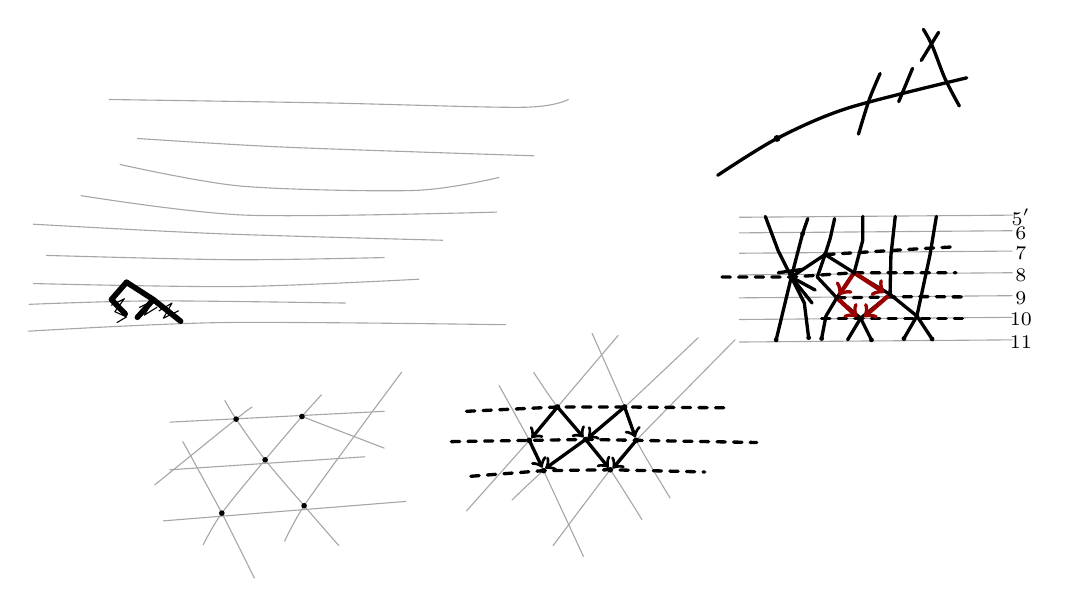
\begin{tikzpicture}[x=.55cm,y=-.55cm,line cap=round,line join=round,g/.style={olive!80!yellow,line width=1.7pt},r/.style={orange!80!brown,line width=1.8pt},w/.style={red!60!black,line width=1.5pt},b/.style={blue!60!black,line width=1.4pt},p/.style={gray!70,thin},k/.style={black,line width=1.2pt},every node/.style={font=\scriptsize}]
% Pencil separators behind the main orders and dark redrawings of lower arrows.
\draw[p] plot[smooth] coordinates {(7.95,8.4) (13.0,8.48) (17.5,8.58) (18.55,8.4)};
\draw[p] plot[smooth] coordinates {(8.6,9.3) (12.0,9.5) (17.75,9.7)};
\draw[p] plot[smooth] coordinates {(8.2,9.9) (11.0,10.4) (15.0,10.5) (16.95,10.2)};
\draw[p] plot[smooth] coordinates {(7.3,10.62) (11.1,11.07) (16.9,11.0)};
\draw[p] plot[smooth] coordinates {(6.2,11.28) (10.5,11.5) (15.65,11.65)};
\draw[p] plot[smooth] coordinates {(6.5,12.0) (10.8,12.1) (14.3,12.05)};
\draw[p] plot[smooth] coordinates {(6.2,12.65) (10.9,12.72) (15.1,12.55)};
\draw[p] plot[smooth] coordinates {(6.1,13.13) (9.0,13.05) (13.4,13.1)};
\draw[p] plot[smooth] coordinates {(6.08,13.75) (10.6,13.55) (17.1,13.6)};
\draw[k,line width=2pt] (8.35,12.62)--(8.0,13.02)--(8.32,13.35);
\draw[k,line width=2pt] (8.35,12.62)--(8.97,13.02)--(8.6,13.43);
\draw[k,line width=2pt] (8.97,13.02)--(9.6,13.52);
\draw[k,thin] (8.0,13.15)--(8.3,13.0)--(8.08,13.3)--(8.35,13.42)--(8.13,13.55);
\draw[k,thin] (8.65,13.2)--(8.96,13.05)--(8.76,13.38)--(9.05,13.2);
\draw[k,thin] (9.1,13.28)--(9.4,13.1)--(9.2,13.45)--(9.55,13.28);
% Upper-right marked line and small crossing.
\draw[k] plot[smooth] coordinates {(22.0,10.15) (23.37,9.3) (25.0,8.6) (27.75,7.9)};
\draw[k] plot[smooth] coordinates {(25.25,9.2) (25.5,8.4) (25.75,7.8)};
\draw[k] plot[smooth] coordinates {(26.18,8.45) (26.5,7.68)};
\draw[k] plot[smooth] coordinates {(26.75,6.78) (26.95,7.15) (27.25,7.92) (27.58,8.55)};
\draw[k] plot[smooth] coordinates {(26.7,7.5) (27.1,6.85)};
\fill[k] (23.37,9.3) circle (.08);
% Middle-right partial grid and darker diagonal paths.
\draw[p] (22.5,11.12)--(28.8,11.069999999999999);
\node at (29.0,11.12) {$5'$};
\draw[p] (22.5,11.48)--(28.8,11.43);
\node at (29.0,11.48) {$6$};
\draw[p] (22.5,11.95)--(28.8,11.899999999999999);
\node at (29.0,11.95) {$7$};
\draw[p] (22.5,12.45)--(28.8,12.399999999999999);
\node at (29.0,12.45) {$8$};
\draw[p] (22.5,12.98)--(28.8,12.93);
\node at (29.0,12.98) {$9$};
\draw[p] (22.5,13.48)--(28.8,13.43);
\node at (29.0,13.48) {$10$};
\draw[p] (22.5,14.0)--(28.8,13.95);
\node at (29.0,14.0) {$11$};
\draw[k] (23.1,11.1)--(23.4,11.9)--(23.7,12.5)--(24.0,13.1)--(24.1,13.9);
\draw[k] (24.08,11.15)--(23.96,11.5)--(23.7,12.5)--(23.35,13.95);
\draw[k] (24.7,11.15)--(24.6,11.6)--(24.48,11.98)--(24.3,12.5)--(24.75,12.98)--(25.3,13.45)--(25.55,13.95);
\draw[k] (25.35,11.1)--(25.35,11.65)--(25.15,12.4)--(24.75,12.98)--(24.5,13.4)--(24.4,13.92);
\draw[k] (26.1,11.1)--(26.0,12.0)--(25.98,12.9)--(25.3,13.45)--(25.0,13.95);
\draw[k] (27.05,11.1)--(26.9,12.0)--(26.6,13.4)--(26.95,13.93);
\draw[k] (23.7,12.5)--(24.48,11.98)--(25.15,12.4)--(25.98,12.9)--(26.6,13.4)--(26.3,13.92);
\draw[k,dashed] (22.1,12.5)--(23.7,12.5)--(25.15,12.4)--(27.5,12.4);
\draw[k,dashed] (24.5,11.98)--(26.6,11.85)--(27.5,11.8);
\draw[k,dashed] (24.75,12.98)--(26.6,12.95)--(27.8,12.96);
\draw[k,dashed] (24.4,13.45)--(25.3,13.45)--(27.65,13.45);
\draw[w,->] (25.15,12.4)--(24.8,12.92);
\draw[w,->] (25.15,12.4)--(25.85,12.86);
\draw[w,->] (24.75,12.98)--(25.22,13.42);
\draw[w,->] (25.98,12.9)--(25.38,13.42);
\fill[k] (23.96,11.5) circle (.055);
\fill[k] (23.7,12.5) circle (.055);
\fill[k] (24.48,11.98) circle (.055);
\fill[k] (25.15,12.4) circle (.055);
\fill[k] (24.75,12.98) circle (.055);
\fill[k] (25.98,12.9) circle (.055);
\fill[k] (25.3,13.45) circle (.055);
\fill[k] (26.6,13.4) circle (.055);
\fill[k] (23.35,13.95) circle (.055);
\fill[k] (24.1,13.9) circle (.055);
\fill[k] (24.4,13.92) circle (.055);
\fill[k] (25.55,13.95) circle (.055);
\fill[k] (26.3,13.92) circle (.055);
\fill[k] (26.95,13.93) circle (.055);
\draw[k] (23.4,12.4)--(23.98,12.32);
\draw[k] (23.7,12.5)--(24.25,12.8);
\draw[k] (23.7,12.5)--(24.18,13.1);
% Bottom middle pencil crossing arrangement.
\draw[p] plot[smooth] coordinates {(9.35,15.85) (14.3,15.6)};
\draw[p] plot[smooth] coordinates {(9.35,16.95) (13.85,16.65)};
\draw[p] plot[smooth] coordinates {(9.2,18.13) (14.8,17.68)};
\draw[p] plot[smooth] coordinates {(9.65,16.3) (10.55,17.95) (11.3,19.45)};
\draw[p] plot[smooth] coordinates {(10.62,15.35) (10.88,15.78) (11.55,16.72) (12.45,17.78) (13.25,18.7)};
\draw[p] plot[smooth] coordinates {(12.85,15.22) (12.4,15.72) (11.55,16.72) (10.55,17.95) (10.12,18.68)};
\draw[p] plot[smooth] coordinates {(14.7,14.7) (13.7,16.05) (12.45,17.78) (12.0,18.6)};
\draw[p] plot[smooth] coordinates {(9.0,17.3) (10.88,15.78) (11.25,15.5)};
\draw[p] plot[smooth] coordinates {(12.4,15.72) (14.3,16.45)};
\fill[k] (10.88,15.78) circle (.065);
\fill[k] (12.4,15.72) circle (.065);
\fill[k] (11.55,16.72) circle (.065);
\fill[k] (10.55,17.95) circle (.065);
\fill[k] (12.45,17.78) circle (.065);
% Bottom-right local arrangement with arrows between three dashed levels.
\draw[p] plot[smooth] coordinates {(16.2,17.9) (17.65,16.27) (18.3,15.5) (19.7,13.85)};
\draw[p] plot[smooth] coordinates {(17.75,14.7) (18.3,15.5) (18.95,16.25) (19.52,16.95) (20.25,18.1)};
\draw[p] plot[smooth] coordinates {(19.1,13.8) (19.85,15.5) (20.12,16.27) (20.9,17.6)};
\draw[p] plot[smooth] coordinates {(16.95,15.0) (17.65,16.27) (17.98,16.97) (18.9,18.95)};
\draw[p] plot[smooth] coordinates {(17.25,17.65) (17.98,16.97) (18.95,16.25) (19.85,15.5) (21.55,13.9)};
\draw[p] plot[smooth] coordinates {(18.2,18.7) (19.52,16.95) (20.12,16.27) (22.4,13.95)};
\draw[k,dashed] (16.2,15.6)--(18.3,15.5)--(19.85,15.5)--(22.25,15.52);
\draw[k,dashed] (15.85,16.3)--(18.95,16.25)--(20.12,16.27)--(22.9,16.32);
\draw[k,dashed] (16.3,17.1)--(17.98,16.97)--(19.52,16.95)--(21.7,17.0);
\draw[k,->] (18.3,15.5)--(17.7,16.22);
\draw[k,->] (18.3,15.5)--(18.9,16.2);
\draw[k,->] (19.85,15.5)--(19.0,16.22);
\draw[k,->] (19.85,15.5)--(20.1,16.2);
\draw[k,->] (17.65,16.27)--(17.95,16.9);
\draw[k,->] (18.95,16.25)--(18.02,16.92);
\draw[k,->] (18.95,16.25)--(19.48,16.9);
\draw[k,->] (20.12,16.27)--(19.58,16.92);
\fill[k] (18.3,15.5) circle (.065);
\fill[k] (19.85,15.5) circle (.065);
\fill[k] (17.65,16.27) circle (.065);
\fill[k] (18.95,16.25) circle (.065);
\fill[k] (20.12,16.27) circle (.065);
\fill[k] (17.98,16.97) circle (.065);
\fill[k] (19.52,16.95) circle (.065);
\end{tikzpicture}}
\diagram{\begin{tikzcd}[ampersand replacement=\&,column sep=.8em,row sep=1em]
\bullet\arrow[dr]\&{}\&\bullet\arrow[dl]\&\bullet\arrow[dr]\&{}\&\bullet\arrow[dl]\\
{}\&{}\arrow[drr]\&{}\&{}\&{}\arrow[dl]\&{}\\
{}\&{}\&{}\&{}\arrow[dl]\&{}\&{}\\
{}\&{}\&{}\arrow[dl]\&{}\&{}\&{}\\
{}\&{}\&{}\&{}\&{}\&{}
\end{tikzcd}}
\margin{\mspage{144}}
